\documentclass[11pt,a4paper]{ivoa}
\input tthdefs

\usepackage{xspace}
% Standard terms used throughout the document,
% defined as macro commands to maintain consistency
% and avoid repeated spelling mistakes.

% Using non-breaking space character.
% https://stackoverflow.com/a/1012891

\usepackage[super]{nth}

\newcommand{\xml} {XML}
\newcommand{\json} {JSON}
\newcommand{\yaml} {YAML}
\newcommand{\http} {HTTP}
\newcommand{\rest} {REST}

\newcommand{\openapi} {OpenAPI}
\newcommand{\datamodel} {data~model}
\newcommand{\webservice} {web service}
\newcommand{\webbrowser} {web browser}

\newcommand{\vo} {VO}
\newcommand{\vofull} {Virtual Observatory}
\newcommand{\ivoa} {IVOA}
\newcommand{\ivoafull} {International Virtual Observatory Alliance}
\newcommand{\uws} {UWS}
\newcommand{\vospace} {VOSpace}

\newcommand{\execworkerclass} {**ExecutionWorker**}
\newcommand{\execbrokerclass} {\textit{ExecutionBroker}}
\newcommand{\execbrokerservice}[1] {\textit{ExecutionBroker~service#1}}

\newcommand{\execoffer}[1] {\textit{ExecutionBroker~offer#1}}
\newcommand{\execofferset}[1] {\textit{ExecutionBroker~offerset#1}}
\newcommand{\execsession}[1] {\textit{ExecutionBroker~session#1}}

\newcommand{\executionbroker} {\textit{Execution~Broker}}
\newcommand{\executionplanning} {\textit{Execution~Planning}}

\newcommand{\executable} {\textit{executable}}
\newcommand{\executablething}[1] {\textit{executable~thing#1}}
\newcommand{\excutabletask} {\textit{executable} task}

\newcommand{\metadoc} [1]{\textit{metadata document#1}}

%\newcommand{\execoffer}[1] {\textit{offer#1}}
\newcommand{\workerjob}[1] {\textit{session#1}}
\newcommand{\teardown} {tear-down}

\newcommand{\jupyter} {Jupyter}
\newcommand{\jupyterhub} {JupyterHub}
\newcommand{\binderhub} {BinderHub}
\newcommand{\jupyternotebook} {Jupyter notebook}

\newcommand{\esap} {ESAP}
\newcommand{\escape} {ESCAPE}
\newcommand{\datalake} {DataLake}
\newcommand{\rucio} {Rucio}

\newcommand{\python} {Python}
\newcommand{\pythonprogram} {Python program}
\newcommand{\pythonruntime} {Python runtime}

\newcommand{\apache} {Apache}
\newcommand{\spark} {Spark}
\newcommand{\pyspark} {PySpark}
\newcommand{\zeppelin} {Zeppelin}
\newcommand{\zeppelinnotebook} {Zeppelin notebook}

\newcommand{\oci} {OCI}
\newcommand{\ociruntime} {OCI runtime}
\newcommand{\ocicontainer} {OCI container}
\newcommand{\docker} {Docker}
\newcommand{\dockercompose} {Docker compose}
\newcommand{\dockerruntime} {Docker runtime}
\newcommand{\dockercontainer} {Docker container}

\newcommand{\singularity} {Singularity}
\newcommand{\singularitycontainer} {Singularity container}

\newcommand{\openstack} {Openstack}
\newcommand{\kubernetes} {Kubernetes}

\newcommand{\codeword}[1] {\texttt{#1}}
\newcommand{\footurl}[1] {\footnote{\url{#1}}}

\newcommand{\dataset}[1] {dataset#1}
\newcommand{\datascience} {data~science}
\newcommand{\scienceplatform}[1] {science~platform#1}

\newcommand{\science}[1] {science#1}
\newcommand{\scientist}[1] {scientist#1}

\newcommand{\cpu}[1] {CPU#1}
\newcommand{\gpu}[1] {GPU#1}
\newcommand{\nvidiagpu} {NVIDIA~AD104~GPU}

\newcommand{\scalable} {scalable}

% TODO add a citation for the YAML specification.
% https://yaml.org/spec/

\usepackage{listings}
\usepackage{xcolor}

%\colorlet{punct}{red!60!black}
\colorlet{numb}{magenta!60!black}
\definecolor{html-gray}{HTML}{EEEEEE}
\definecolor{light-gray}{gray}{0.95}
\definecolor{delim}{RGB}{20,105,176}

\lstset{
    basicstyle=\small\ttfamily,
    columns=fullflexible,
    frame=none,
    backgroundcolor=\color{light-gray},
    stepnumber=1,
    %numbers=left,
    numbers=none,
    numberstyle=\small,
    numbersep=8pt,
    %xleftmargin=\parindent,
    xrightmargin=1cm,
    showstringspaces=false,
    keepspaces=true,
    breaklines=true,
    linewidth=14cm,
    frame=none
}

% https://tex.stackexchange.com/questions/83085/how-to-improve-listings-display-of-json-files
% https://tex.stackexchange.com/a/83100
% https://tex.stackexchange.com/questions/10828/indent-a-code-listing-in-latex
% https://tex.stackexchange.com/a/10831
\lstdefinelanguage{json}{
    literate=
     *{0}{{{\color{numb}0}}}{1}
      {1}{{{\color{numb}1}}}{1}
      {2}{{{\color{numb}2}}}{1}
      {3}{{{\color{numb}3}}}{1}
      {4}{{{\color{numb}4}}}{1}
      {5}{{{\color{numb}5}}}{1}
      {6}{{{\color{numb}6}}}{1}
      {7}{{{\color{numb}7}}}{1}
      {8}{{{\color{numb}8}}}{1}
      }

\lstdefinelanguage{yaml}{
    literate=
     *{0}{{{\color{numb}0}}}{1}
      {1}{{{\color{numb}1}}}{1}
      {2}{{{\color{numb}2}}}{1}
      {3}{{{\color{numb}3}}}{1}
      {4}{{{\color{numb}4}}}{1}
      {5}{{{\color{numb}5}}}{1}
      {6}{{{\color{numb}6}}}{1}
      {7}{{{\color{numb}7}}}{1}
      {8}{{{\color{numb}8}}}{1}
      }

\hyphenation{Exe-cut-able-Thing}

\title{IVOA Execution Broker}

% see ivoatexDoc for what group names to use here; use \ivoagroup[IG] for
% interest groups.
\ivoagroup{GWS}

\author[http://www.ivoa.net/twiki/bin/view/IVOA/DaveMorris]
       {Dave Morris}
\author[http://www.ivoa.net/twiki/bin/view/IVOA/SaraBertocco]
       {Sara Bertocco}

\editor[http://www.ivoa.net/twiki/bin/view/IVOA/DaveMorris]
       {Dave Morris}

% \previousversion[????URL????]{????Concise Document Label????}
\previousversion{This is the first public release}

\begin{document}
\begin{abstract}
\label{abstract}

One of the long term goals of the \ivoa{} has been to enable users to
move the code to the data.
This is becoming more and more important as the size and complexity
of the \dataset{s} available in the virtual observatory increases.
%\citep{gaia-at-esac}
%\footurl{https://www.skao.int/en/explore/big-data}
%\footurl{https://www.lsst.org/scientists/keynumbers}

The \ivoa{} \executionbroker{} provides a step towards making this possible.

The \ivoa{} \executionbroker{} is designed to address a specific question;
given an executable thing, e.g. a \pythonprogram{} or \jupyternotebook{}.
What facilities are available to run it?

To do this, the \ivoa{} \executionbroker{} specification defines
a \datamodel{} and \webservice{} API for describing executable things
and the resources needed to execute them.

Together these components enable a user to ask a simple question
\textit{"Where (and when) can I execute my program?"}

This in turn enables users to move code between \scienceplatform{s}.
Allowing them to develop their code on one platform and then apply it to a different
\dataset{} by sending it to execute on another platform.

\end{abstract}

\section*{Acknowledgments}
\label{acknowledgments}

The authors would like to thank all the participants in the IVOA and ESCAPE projects
who have contributed their ideas, critical reviews, and suggestions to this document.

\section*{Conformance-related definitions}

The words ``MUST'', ``SHALL'', ``SHOULD'', ``MAY'', ``RECOMMENDED'', and
``OPTIONAL'' (in upper or lower case) used in this document are to be
interpreted as described in IETF standard RFC2119 \citep{std:RFC2119}.

The \emph{Virtual Observatory (VO)} is a general term for a collection of
federated resources that can be used to conduct astronomical research,
education, and outreach.
The \href{https://www.ivoa.net}{International Virtual Observatory Alliance (IVOA)}
is a global collaboration of separately funded projects to develop standards and
infrastructure that enable VO applications.

\section{Introduction}
\label{introduction}

The \ivoa{} \executionbroker{} specification defines a \datamodel{} for describing executable tasks
and a \webservice{} interface for managing them.
Together these provide a common interface for service discovery, resource allocation
and execution scheduling across a heterogeneous federation of different types of
execution platform.

\begin{itemize}
    \item \execbrokerclass{} \datamodel{}  – a data model for describing execution sessions and their resource requirements.
    \item \execbrokerclass{} \webservice{} – a \rest{} based web service to find execution platforms, allocate resources and schedule execution sessions.
\end{itemize}

\subsection{Role within the VO Architecture}
\label{subsec:ivoarole}

% As of ivoatex 1.2, the architecture diagram is generated by ivoatex in
% SVG; copy ivoatex/archdiag-full.xml to role_diagram.xml and throw out
% all lines not relevant to your standard.
% Notes don't generally need this.  If you don't copy role_diagram.xml,
% you must remove role_diagram.pdf from SOURCES in the Makefile.
\begin{figure}
\centering
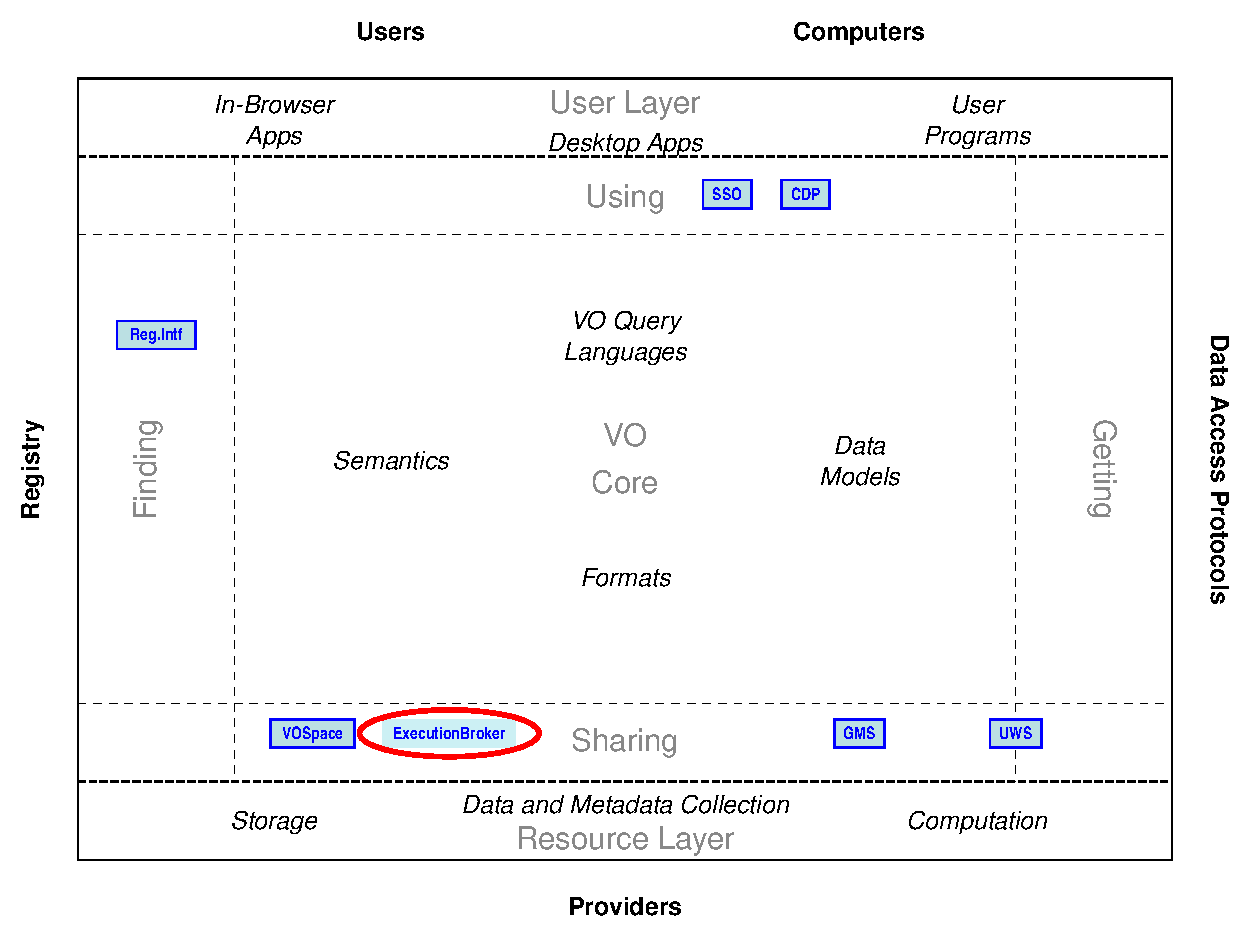
\includegraphics[width=0.9\textwidth]{role_diagram.pdf}
\caption{Architecture diagram showing the \ivoa{} \executionbroker{}'s role in the \ivoa}
\label{fig:archdiag}
\end{figure}

The \ivoa{} Architecture\citep{2010ivoa.rept.1123A} provides a high-level view of how \ivoa{}
standards work together to connect users and applications with providers of data
and services.
Fig.~\ref{fig:archdiag} shows the role the \ivoa{} \executionbroker{} plays within this architecture.

In response to the increasing size and complexity of the next generation of science \dataset{s}
a number of \ivoa{} members are developing intergrated \scienceplatform{s} which bring
together the \dataset{s} co-located with the compute resources needed to analyse
them.\footurl{https://data.lsst.cloud/}\footurl{https://rsp.lsst.io/}

These \scienceplatform{s} make extensive use of the \ivoa{} data models and
vocabularies to describe their \dataset{s}, and use the \ivoa{} data access
services to find and access data from other data providers.
In addition, some of the \scienceplatform{s} use \ivoa{} \vospace{} services to manage
data transfers to and from local storage co-located with the compute resources.

However, to date the \ivoa{} does not provide any APIs or services that
enable \scienceplatform{s} to exchange the software used to analyse the data.
The \ivoa{} \executionbroker{} provides a step towards making this possible.

This places the \ivoa{} \executionbroker{} in the same region of the \ivoa{} architecture
as the \ivoa{} \vospace{} specification \citep{2009ivoa.specQ1007G},
providing an infrastructure level service that enables service discovery,
resource allocation and execution scheduling across a heterogeneous federation
of execution platforms.

\subsection{Supplementary documents}
\label{supplementary-documents}

\subsubsection{\openapi{} specification}
\label{openapi-specification}

This document is designed to read in combination with the \openapi{}
\footurl{https://www.openapis.org/} \footurl{https://swagger.io/specification/}
specification published alongside this document.

The \openapi{} specification defines the technical details of the
\executionbroker{} \webservice{} interface and the schema for the
\executionbroker{} \datamodel{}.
This document compliments the technical specification by using use cases
and specific examples to describe the intended service behaviour and
explain the reasoning behind some of the design choices.

The two documents are intended to be read together.
The machine-readable \openapi{} spcification defining the \textit{what},
and the human-readable text document describing the \textit{why}.

The \openapi{} specification associated with this document is
published in the following files:
\begin{itemize}
    \item \codeword{openapi.yaml} - The main service specification, including
    the \executionbroker{} service API and the core data model.
    \item \codeword{messages.yaml} - a supplimentary data model for INFO, WARN,
    and DEBUG messages embedded in the service responses.
    \item \codeword{utils.yaml} - a supplimentary data model for re-usable
    components such as ISO date formats, min/max pairs, and name-value maps.
\end{itemize}

This text document may include small examples of \openapi{} schema to
explain specific points, but these are for information only. Unless otherwise
specified, the \openapi{} specification itself should be assumed to be the
definitive source and this text document should be considered as secondary.

\subsubsection{IVOA profiles}
\label{ivoa-profiles}

This specification refers to the following documents
to cover the details of how an \executionbroker{} \webservice{}
should use the following protocols and data formats:
\begin{itemize}
    \item The \ivoa{} \rest{} profile, describing a common pattern
    for \ivoa{} \webservice{s} that implement
    \rest{}\footurl{https://en.wikipedia.org/wiki/REST}
    webservices.
    \item The \ivoa{} \http{} profile, describing how \ivoa{} \webservice{s}
    should use aspects of the \http{} protocol, including \http{} parameters,
    message content, content negotiation, and \http{} return codes.
    \item The \ivoa{} error messages profile, describing a common format
    for \ivoa{} \webservice{s} to format error messages.
    \item The \ivoa{} \json{} profile, describing how \ivoa{} \webservice{s}
    should serialize message content using the
    \json{}\footurl{https://www.json.org/json-en.html} data format.
    \item The \ivoa{} \yaml{} profile, describing how \ivoa{} \webservice{s}
    should serialize message content using the
    \yaml{}\footurl{https://yaml.org/} data format.
    \item The \ivoa{} \xml{} profile, describing how \ivoa{} \webservice{s}
    should serialize message content using the
    \xml{}\footurl{https://www.w3.org/XML/} data format.
\end{itemize}

Unless otherwise specified, an \executionbroker{} \webservice{} implementation
should follow the guidelines outined in these documents.

\subsubsection{IVOA Single-Sign-On}
\label{ivoa-sso}

In addition, an \ivoa{} \executionbroker{} service may use parts of the
\ivoa{} Single-Sign-On standard\citep{2017ivoa.spec.0524T}
for authentication, and the
\ivoa{} Credential Delegation Protocol \citep{2010ivoa.spec.0218P}
for delegating credentials to other services.

\subsection{Executable things}
\label{executablething}

To understand the problem that the \ivoa{} \executionbroker{} is trying to solve
it is useful to describe what an \executablething{} is in this context.
In general terms, this document refers to something that can be executed, or run,
as an \executable{}.

To explain what this means we can start with a science domain function that we want to perform.
For example, the mathematical concept of the square root of a number.
We can calculate the square root of a positive number using the Newton–Raphson
algorithm\footurl{https://en.wikipedia.org/wiki/Newton\%27s_method}
which produces successively closer approximations to the result.
However, in general case, this mathematical description of the algorithm would not be
considered to be an \executablething{}.

We can write a \pythonprogram{} to use this algorithm to calculate the square root of a number.
This is the first identifiable \executablething{} in our example.
To be able to use this \executablething{}, you would need a computing resource with the appropriate
hardware and software environment. In this case, a computing resource with the \python{} interpreter
installed along with the additional \python{} modules required by the program.
This environment is often referred to as the \python{} runtime.

In the context of \scienceplatform{s} and \datascience{}, a common pattern is to provide this environment
using a Docker\footurl{https://docs.docker.com/get-started/what-is-a-container/}
or OCI\footurl{https://opencontainers.org/} container
to package the \pythonprogram{} and \python{} runtime together as a single binary object.
This package, or container, is itself an \executablething{}. One which requires a different execution
environment than the original \pythonprogram{}.
The aim of containerization is to package software components together with all the libraries and dependencies
they need as a single binary object that interfaces with a standard execution environment,
referred to as the \textit{container runtime}.
To be able to use this \executablething{}, you would need a computing resource with the appropriate
hardware and software environment. In this case, a computing resource with the \docker{} or \ocicontainer{}
runtime installed.

We could also create a \jupyternotebook{} that demonstrates how to use our \pythonprogram{}.
This is the third \executablething{} in our example.
One which provides an interactive environment for the user to experiment with.
As before, to be able to use this \executablething{}, we would need a computing resource with
the appropriate hardware and software environment.
In this case, a computer with the \jupyternotebook{} platform installed along with all the \python{} modules
needed by our \pythonprogram{}.
In the context of \scienceplatform{s} and \datascience{}, a common pattern is to provide this environment as a \webservice{}
that allows the user to interact with the \jupyternotebook{} via a \webbrowser.

From one algorithm that implements a science domain function, we have created three different \executablething{s}.
A \pythonprogram{}, a \dockercontainer{} packaging the \pythonprogram{}, and an interactive \jupyternotebook{}
that demonstrates how to use the \pythonprogram{}.
Each of which requires a different computing environment to execute.
A basic \python{} runtime, the \dockerruntime{}, and a \jupyternotebook{} service.

We may also want to consider the data that we are applying the algorithm to and the compute resources that
will be needed to process it.
If we are running some small experiments to learn how to use the algorithm, then a basic computing
resource will probably be sufficient.
However, if we have a \dataset{} of ten million numbers that we want to process, then we may
need to consider adding extra storage to handle the input data and the results.
For a large \dataset{} it may also be worth using a \gpu{} to accelerate the calculation.

The \ivoa{} \executionbroker{} \datamodel{} provides a way to describe what each of these \executablething{s}
are and what resources are needed to execute them.
This can include things like number of \cpu{} cores and amount of memory it needs,
whether it needs a \gpu{}, the location of the input data, the storage space needed to perform
the calculation, and the storage space needed to save the results.

\section{Service interaction}
\label{service-interaction}

The interaction between a user, the client application they are using, and the services available in the \vo{}
can be described as a conversation between the client and one or more \execbrokerservice{s} to discover
where, how, and when, an \executablething{} can be executed.

\subsection{Discovery services}
\label{discovery-services}

The conversation starts at the discovery stage, where the user uses discovery services to
select the software and \dataset{s} that they want to work with.

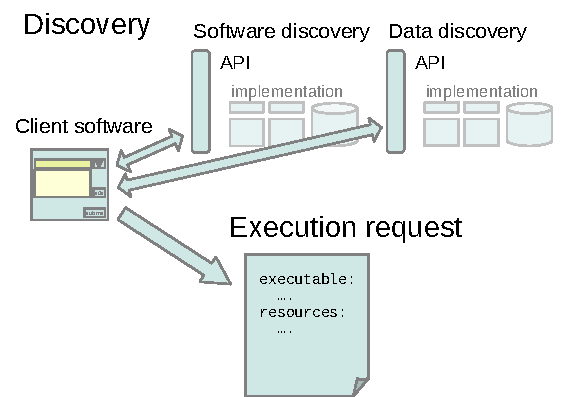
\includegraphics[width=0.9\textwidth]{diagrams/data-discovery.pdf}

The detailed specification for the software and data discovery services are beyond the
scope of this document. However we can outline some general requirements for them.

In both cases, the discovery process should not depend on the technical details
of the software or the \dataset{s}, but on their science domain functionality and properties.

From a science user's perspective they want to be able to find software that implements
a particular clustering algorithm, or a \dataset{} that is indexed according to a particular
coordinate system.
The programming language the software is written in and the file format of the \dataset{}
are at best secondary criteria.
In our square root example, we would expect our user to use search terms like \textit{'square root'}
or \textit{'newton raphson'} to find the software they need.
We wouldn't expect them to start out looking for a \textit{'python'} or \textit{'docker'} as their key search terms.
Ideally, if the \executionbroker{} service functions as intended, a science user should not
need to know about programming languages, software packaging or file formats.
The \executionbroker{} service should hide as much as possible of the technical details,
enabling the science user to get on with science.

Another important consideration is these discovery services should be designed to be domain agnostic.
Meaning that it should be possible to swap out an astronomy based discovery service
for an equivalent biochemistry discovery service and although the domain specific
terms and vocabulary will be different, the techical details of the service interfaces
should be the same.

\subsubsection{Software discovery}
\label{software-discovery}

There are three main components involved in software discovery, the metadata schema for
describing the software, one or more search services, and the
repositories where the \executablething{s} are stored.

The vocabularies and schema need to be based on use cases that start by describing what the
\scientist{} wants to do, and from that derrive what software tools they would need, and what terms
they would naturally use to describe them.

The \ivoa{} semantics and data modelling working groups have a lot of experience developing
vocabularies and data models to descibe \science{} data products, and is well placed
to develop the vocabularies needed to descibe astronomy software.

It is important to keep in mind that the requirement is not to model the technical properties
of the software itself e.g. what programming language it is written in or who funded the development.
The important things to model are the search terms that a \scientist{} is most likley to use to try to
find the software they need.

The second component is a searchable database that acceopts a list of search terms and responds with a
list of \metadoc{s} that describe \executablething{s} that match the criteria.

Before we look in detail at the content of the \metadoc{s} it is worth looking at where the \metadoc{s} are
stored in relation to the search service and the repositories where the \executablething{s} are stored.

In one scenario, all of the components can be co-located by the same service.
The database of search terms, the \metadoc{s}, and the binary files containing the \executablething{s}
can all be hosted by the same service implementation.

TODO diagram

An alternative implementation could store them at different locations, using
existing off-the-shelf software and services to host them.

There are a number of widely available content managment systems, both commercial
and open source, that would be capable of implementing the database of search terms.

If the \metadoc{s} are stored in the same database, then the response from a
database search could contain the \metadoc{s} themselves.

TODO diagram
database, results, contain \metadoc{s} from database

Alternatively, the \metadoc{s} could be stored at a separate location,
in an online git repository for example,
and the database search response simply contains a list of URLs that
point to the individual \metadoc{s}.

TODO diagram
database, results, links to \metadoc{s} in external repositories

The third part of the set is the binary image of the \executablething{}.
In most cases it would probably make sense for the \metadoc{} to reference
the \executablething{} as a binary file stored in an external repository
rather than trying to include the \executablething{} as a binary blob in
the database.

TODO diagram
database, results, links to \metadoc{s} with links to images

The system can use standard cryptographic signatures and checksums to ensure the validity
of the \metadoc{s} and the binary images they refer to even when they are stored and accesed
via external \nth{3} party services.

In summary, there are two things that need to be standardised for a software discovery service:
\begin{itemize}
    \item The inputs to the discovery service, including the metadata vocabularies
        used to describe the software in terms that make sense to the \scientist{}
        looking for them. For example what algorithm it implements, the type of input data it
        operates on, and the type of results it generates.
    \item The outputs of the discovery service, including the \metadoc{s} defined by this
        specification, that describe the binary images that package the software
        as \executablething{s}.
\end{itemize}

The other components in the software discovery stack, the database of search terms, and
storage and access services for the \metadoc{s} and binary images, do not need to be
standardised at this stage.

\subsubsection{Data discovery}
\label{data-discovery}

TODO : update this with reference to \ivoa{} data product type.
https://www.ivoa.net/rdf/product-type/2024-05-19/product-type.html

\subsection{Execution broker}
\label{execution-broker-intro}

\subsubsection{OfferSet request}
\label{offerset-request}

Once the user has selected the \executablething{} they want to use and the
data they want to apply it to, the client combines this information to create a
complete description of the \execsession{} the user wants to execute, including
details of the executable, the compute, storage, and data resources it needs,
and a schedule describing when the user wants it to run.

\begin{lstlisting}[]
# ExecutionBroker OfferSet request.
executable:
  ....
resources:
  ....
schedule:
  ....
\end{lstlisting}

The client sends the \metadoc{} description to one or more \execbrokerclass{}
services to ask if they can meet the requirements and execute the \execsession{}.

Each \execbrokerservice{} evaluates the request and responds with a top level
\codeword{YES|NO} answer, and if
the answer is \codeword{YES}, a list of one or more \execoffer{s} describing how
the requested \execsession{} could be executed on the platform(s) represented by
that \execbrokerservice{}.

%\begin{lstlisting}[]
%Request  - Can this platform execute <task> ?
%Response - YES, list of <offer>[]
%\end{lstlisting}

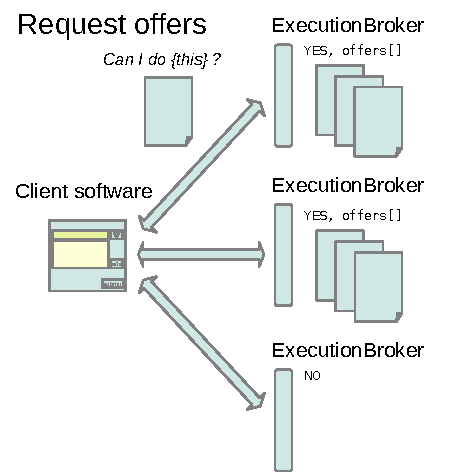
\includegraphics[width=0.9\textwidth]{diagrams/request-offers.pdf}

\subsubsection{Offerset response}
\label{offerset-response}

Each \execbrokerservice{} will respond to a request for offers with an \execofferset{}
containing some metadata about the \execofferset{} itself, and a list of \execoffer{}s
describing how the requested \execsession{} could be executed.

Each \execoffer{} in the list contains some metadata about the \execoffer{} itself,
including its UUID identifier and expiry time, followed by details of how and when the
\execsession{} would be executed.

\begin{lstlisting}[]
# ExecutionBroker OfferSet response.
result: YES
....
offers:

- uuid: "2e164a1b-7ff6-11ef-8412-4bc36fe2face"
  href: "http://..../sessions/2e164a1b-7ff6-11ef-8412-4bc36fe2face"
  state: 'OFFERED'
  expires: "2023-09-18T07:05:21"
  ....
  executable:
    ....
  resources:
    ....
  schedule:
    ....

- uuid: "2e16bf4c-7ff6-11ef-8412-4bc36fe2face"
  href: "http://..../sessions/2e16bf4c-7ff6-11ef-8412-4bc36fe2face"
  status: 'OFFERED'
  expires: "2023-09-18T07:05:21"
  ....
  executable:
    ....
  resources:
    ....
  schedule:
    ....
\end{lstlisting}

The user can choose to accept one of the \execoffer{s} from the list that best
fits their requirements, or they can reject the \execoffer{s} and make a new
request with different criteria.

Each of the \execoffer{s} in the \execofferset{} represent a temporary reservation
for the resources listed in the \execoffer{}.
This means these resources will not available to other users while the \execoffer{s}
are still valid.

If the user does nothing, then \codeword{state} of each of the \execoffer{s} will
automatically be updated to \codeword{EXPIRED}, and their associated resources will
be released, when their expiry time is reached.

If the user accepts one of the \execoffer{s} in the \execofferset{} by updating
the \codeword{state} to \codeword{ACCEPTED}, the \execbrokerservice{} SHOULD
update the \codeword{state} of the other \execoffer{s} in the \execofferset{} to
\codeword{REJECTED} and release the associated resources.

TODO [accept/reject/expire state-transition diagram ]

\subsubsection{Update options}
\label{update-options}

Each \execsession{} has a unique URL that the client can use to monitor and update
its state.

The \execbrokerservice{} response for an \execsession{} includes a list of options
that the user may use to update or modify the \execsession{}.
Which options are available will depend on the current \codeword{state} of the
\execsession{} and the identity and permissions of the authenticated user.

If the \execsession{} is still being offered, then the list of available options
allow the user to accept or reject the offer by updating the \codeword{state} of
the \execsession{} to \codeword{ACCEPTED} or \codeword{REJECTED}.

\begin{lstlisting}[]
uuid: "2e164a1b-7ff6-11ef-8412-4bc36fe2face"
href: "http://..../sessions/2e164a1b-7ff6-11ef-8412-4bc36fe2face"
state: 'OFFERED'
expires: "2023-09-18T07:05:21"
....
....
options:
  - type: "uri:enum-value-option"
    path: "state"
    values:
    - "ACCEPTED"
    - "REJECTED"
\end{lstlisting}

Once the \execoffer{} has been accepted and the \execsession{} has started to
execute, then the list of available options will only allow the user to cancel
the execution.

\begin{lstlisting}[]
uuid: "2e164a1b-7ff6-11ef-8412-4bc36fe2face"
href: "http://..../sessions/2e164a1b-7ff6-11ef-8412-4bc36fe2face"
state: 'ACCEPTED'
expires: "2023-09-18T07:05:21"
....
....
options:
  - type: "uri:enum-value-option"
    path: "state"
    values:
    - "CANCELLED"
\end{lstlisting}

Using a dynamic list of options in this way enables the \execbrokerservice{}
to communicate to the client what actions the user is able to take
over the lifetime of an \execsession{}.

\subsection{Session lifecycle}
\label{session-lifecycle}

A \workerjob{} in an \execworkerclass{} service goes through the following stages in its lifecycle.

\begin{itemize}

    \item \codeword{OFFERED}    The \workerjob{} is being offered.
    \item \codeword{ACCEPTED}   The \workerjob{} has been accepted.
    \item \codeword{REJECTED}   The \workerjob{} offer has been rejected.
    \item \codeword{EXPIRED}    The \workerjob{} offer has expired.
    \item \codeword{WAITING}    The \workerjob{} is waiting to activate.
    \item \codeword{PREPARING}  The resources are being prepared.
    \item \codeword{READY}      The \workerjob{} is ready to execute.
    \item \codeword{RUNNING}    The \workerjob{} is executing.
    \item \codeword{RELEASING}  The resources are being released.
    \item \codeword{COMPLETED}  The \workerjob{} has completed.
    \item \codeword{CANCELLED}  The \workerjob{} has been cancelled.
    \item \codeword{FAILED}     The \workerjob{} has failed.

\end{itemize}

When a \execbrokerclass{} creates a \workerjob{} in an \execworkerclass{} service the
\workerjob{} starts with the \codeword{phase} set to \codeword{PENDING}.

It is up to the \execworkerclass{} to select the right time to change the \workerjob{}
\codeword{phase} from \codeword{WAITING} to \codeword{PEPARING} and begin preparing the resources so that
the \workerjob{} is \codeword{READY} in time for the \codeword{starttime} declared
in the \execoffer{}.

If it will take 2 hours to transfer the data resources
from archive storage to live storage co-located with the compute resources,
then the \execworkerclass{} needs to start the \codeword{PREPARING} phase at least 2 hours
before the \codeword{starttime} declared in the \execoffer{}.

Once all the resources are ready, the \execworkerclass{} changes the \workerjob{}
\codeword{phase} to \codeword{READY} to indicate that the all the resources
are ready and the \workerjob{} is waiting to start.

The \execworkerclass{} will then wait until the \codeword{starttime} declared in the \execoffer{}
at which point it will start executing the \workerjob{} and change the \workerjob{} \codeword{phase}
to \codeword{RUNNING}.

When the \workerjob{} finishes executing, because the \dockercontainer{} finished executing,
the user closed their \jupyternotebook, or the \codeword{maxduration} was reached,
the \execworkerclass{} will change the \workerjob{} \codeword{phase} to \codeword{TEARDOWN} and
begin the process of releasing the resources.

If the \workerjob{} includes some persistent storage that should last beyond the end of the \workerjob{},
then part of the \teardown{} process may involve transferring results from the \workerjob{}
onto the persistent storage before the local storage is released.

When the \teardown{} process completes, the \workerjob{} \codeword{phase} is changed to \codeword{COMPLETED}.

If an error occurs at any time in the process, the \workerjob{} \codeword{phase} is changed to \codeword{FAILED}.
This includes any errors that occur during the \teardown{} process; for example, because
the \execworkerclass{} was unable to transfer the results onto persistent storage.
Then the \workerjob{} \codeword{phase} is changed to \codeword{FAILED}, even if the main part of the
execution completed successfully.
This is because any workflow steps that follow after this step, will depend not only on the execution being
completed, but they also need the \teardown{} data transfers to complete so that the results from this step
are in the right place for the next step to be able to access them.

\section{The data model}
\label{data-model}

\subsection{Metadata roles}
\label{metadata-roles}

The full description of an \executablething{} will include several layers of metadata
provided by different actors playing different roles within the publishing process.

For our square root example we can identify a number of roles that would each provide
layers of the picture nedeed to fully describe an \executablething{}.

The players:
\begin{itemize}
    \item The developer  - The person who wrote the \pythonprogram{}
    \item The packager   - The person who packaged it in a \dockercontainer{}
    \item The publisher  - The person who published it in a discovery service
    \item The user agent - The person who wants to use the software
\end{itemize}

\subsubsection{The developer}
\label{software-developer}

The first layer of metadata comes from the person who wrote the software.
They have detailed knowledge of what the software does, what execution environment it needs,
and what the inputs and outputs are.

For our square root example, it is a \pythonprogram{} which needs a platform with the \python{} runtime installed,
and a list of the \python{} libraries that the program relies on.

\begin{lstlisting}[]
executable:
  name: Newton-Raphson example
  type: uri:python-program
  requirements:
  - numpi: ""
  - astropy: ">= 6.1"
\end{lstlisting}

The developer also understands how much memory their program needs, whether it can make use of multiple cpu cores,
and whether it can make use of a \gpu accelerator.

\begin{lstlisting}[]
resources:
  compute:
    - type: uri:generic-compute
      cores:
        requested:
          min: 4
      memory:
        requested:
          min: 16
          units: GiB
      ....
\end{lstlisting}

The developers also know about what inputs and outputs the program expects and what file
formats can it can handle.
% needs work
%https://github.com/ivoa-std/ExecutionBroker/issues/89

\begin{lstlisting}[]
executable:
  name: Newton-Raphson example
  type: uri:python-program
  ....
  parameters:
    - name: input data
      type: uri:param-file
      mode: readonly
      description:
        A table containing a list of numbers to be processed, formatted as
        comma separated text (CSV) or an IVOA VOTable.
      formats:
        - type: uri:text-csv
          ....
        - type: uri:votable
          ....
    - name: input column
      type: uri:param-value
      description:
        The column name within the 'input data' to use.
\end{lstlisting}

\subsubsection{The packager}
\label{software-packager}

Although it is possible to publish our square root example as a stand alone \pythonprogram{},
it is not easy to describe the installation process in sufficient detail for it to be
automatically deployed on a range of different platforms.

A more portable solution would be to package the \pythonprogram{} in a \dockercontainer{},
installing and configuring the software along with all of its dependencies inside the container.

This is often done as part of the software development process, but it is a separate
step that could be implemented by a different person.
To make this distinction clear we can refer to this person, or role, as 'the packager'.

This step packages the \pythonprogram{} along with any \python{} modules it requires,
the \pythonruntime{}, and any operating system components it requires, into a single
standard format binary file, making it much easier to deploy.

To represent the new type of \executablething{} in the \metadoc{}, the packager
would change the description of the \executablething{} from a \pythonprogram{}
to a \dockercontainer{}.

\begin{lstlisting}[]
executable:
  name: Newton-Raphson example
  type: uri:docker-container-1.0
  repository: ghcr.io
  image: ivoa/analytics/Newton-Raphson-albert
  tag: 2024.08.30
  ....
\end{lstlisting}

Depending on how the software is packaged in the container they may also need to update
the description of the inputs and outputs, and link them to specific locations in the
filesystem.
% needs work
%https://github.com/ivoa-std/ExecutionBroker/issues/89

\begin{lstlisting}[]
executable:
  name: Newton-Raphson example
  type: uri:docker-container-1.0
  ....
  parameters:
    - name: input-data
      type: uri:data-file
      format:
        - type: uri:ivoa-votable
          filename: input-data.vot
          ....

resources:
  compute:
    - type: uri:generic-compute
      volumes:
        - type: uri:file-mount
          parameter: input-data
          filepath: /data
          mode: readonly
          ....
\end{lstlisting}

\subsubsection{The publisher}
\label{metadata-publisher}

This role represents the person who publishes metadata about the software in a discovery service.

Typically changes made at this level would include adding to the description
of what the software does, placing it in a particular context to aid discovery,
or modifying the execution environment to configure the softweare for a particular domain.

For example, this might include:

\begin{itemize}
    \item A project specific discovery service that only includes software vetted by the project.
          Execution platforms within the project would only accept curated \metadoc{s}
          from that discovery service.
    \item A domain specific discovery service that modifies the execution environment, configuring
          the software to analyse a particular type of data.
    \item A catalog of \metadoc{s} maintained as part of a university teaching course, modifying the
          execution environment to integrate the software into the university system and setting
          parameters to configure it to match the course notes.
\end{itemize}

\subsubsection{The user}
\label{software-user}

The user starts with an initial \metadoc{} from the
software discovery service and adds additional information describing how they
want to use the software.

This would include selecting the data resources that they want to use
and adding them to the metadata.

\begin{lstlisting}[]
executable:
  ....

resources:

  data:
  - name: input data
    type: uri:simple-data-resource
    location: http:data.example.org/....
    filesize:
      value: 145
      units: MiB
    ....

  compute:
    ....
\end{lstlisting}

Including details of the data resources in the \metadoc{} means the \execbrokerservice{}
will include the time needed to transfer the data to local storage before the
\execsession{} is begins.

Including a value for the data size enables the \execbrokerservice{} to estimate
how much local storage it will need to allocate
and how much time will be needed to transfer the data.
The \execbrokerservice{} can take this into account when calculating the start time of
the \execoffer{s} it makes, allowing enough time for the data transfers to complete
before the \execsession{} starts.

Linking the data resources with volumes on the corresponding compute resources enables
the \execbrokerservice{} to mount the data resources at the correct location in
the compute resource's filesystem.

\begin{lstlisting}[]
resources:

  data:
  - name: input-data
    type: uri:simple-data-resource
    location: http:data.example.org/....
    ....

  compute:
  - type: uri:generic-compute
    ....
    volumes:
    - resource: input-data
      path: /data
      mode: "ro"

\end{lstlisting}

The user can also update the compute resource requirements to reflect how they plan
to use the software.
In the case of our square root example, the compute resource requirements set by the
developers will reflect the original intent of simply demonstrating how to use the
\pythonprogram{}.

However, if the user intends to use the software to analyse a much larger \dataset{}
they can update the compute resource requirements to match their use case.

\begin{lstlisting}[]
resources:
  compute:
  - type: uri:generic-compute
    cores:
      requested:
      # min: 4
        min: 32
    memory:
      requested:
      # min: 16
        min: 128
        units: GiB
\end{lstlisting}

TODO user provides the schedule to describe when they want to run it.

\subsection{The \executable{}}
\label{executable}

At the simplest level the client just needs to check whether a platform is able to execute a particular
type of \excutabletask{}.
For example, \textit{"Is this platform able to run a \jupyternotebook{}?"}

In order to do this, the request needs to specify the task type, e.g. \jupyternotebook{},
along with details about it, e.g. where to fetch the notebook from.

The information in this part of the \datamodel{} will be different for each type of \executable{}.
Rather than try to model every possible type of \executable{} in one large \datamodel{},
the \datamodel{} for each type is described in an extension to the core \datamodel{}.

The \datamodel{} uses a common pattern for polymorphic types based on a discriminator
value to indicate the type of thing it is describing, followed by the specific
details for that type.

This is implemented in the \openapi{} specification as an abstract base class
containing common fields like a name and uuid identifier, followed by a list
of derived types and their type identifiers.

\begin{lstlisting}[]
    AbstractExecutable:
      type: object
      discriminator:
        propertyName: type
        mapping:
          "uri:docker-container-1.0":   'DockerContainer'
          "uri:jupyter-notebook-1.0":   'JupyterNotebook'
          ....
      properties:
        name:
          description: >
            A human readable name, assigned by the client.
          type: string
        uuid:
          description: >
            A machine readable UUID, assigned by the server.
          type: string
          format: uuid
        type:
          description: >
            The type identifier.
          type: string
\end{lstlisting}

The derived types extend this abstract base class to include the details needed to
describe this type of \executablething{}.
For example, the derived type for a \dockercontainer{} includes properties
to describe where to get the \docker image from, including the repository endpoint URL,
and the name and version tag of the \docker{} image to download.

\begin{lstlisting}[]
    DockerContainer:
      description: |
        A Docker or OCI container.
        See https://opencontainers.org/
      type: object
      title: DockerContainer
      allOf:
        - $ref: 'AbstractExecutable'
        - type: object
          properties:
            repository:
              type: string
              description: >
                The image respository URL.
            image:
              type: string
              description: >
                The image name within the repository.
            tag:
              type: string
              description: The image tag.
            ....
\end{lstlisting}

This results in the following message being sent to request the execution
of a \dockercontainer{}.

\begin{lstlisting}[]
# ExecutionBroker request.
request:

  # Details of the executable.
  executable:

    # Common fields from the AbstractExecutable
    name: Experiment one
    type: uri:docker-container-1.0

    # The details, specific to a Docker container executable.
    repository: ghcr.io
    image: ivoa/analytics/Newton-Rahpson-example
    tag: 2024.08.30

\end{lstlisting}

\subsubsection{\jupyternotebook{}}
\label{jupyternotebook}
The \datamodel{} for each type of \executable{} defines the metadata needed to
describe that particular type.
For example, the \datamodel{} for a \jupyternotebook{} needs to describe where
to fetch the source code for the notebook from.

% Type URLs
% https://www.purl.org/ivoa.net/executable-types/jupyter-notebook
% https://github.com/ivoa-std/ExecutionBroker/blob/main/types/executable-types/jupyter-notebook.md
\begin{lstlisting}[]
# ExecutionBroker client request.
request:
  # Details of the executable.
  executable:
    # A URI identifying the type of executable.
    type: "https://www.purl.org/ivoa.net/executable-types/jupyter-notebook"

    # The details, specific to a Jupyter notebook.
    spec:
      notebook: "https://.../example.jpnb"
\end{lstlisting}

It may also include a reference to a \codeword{requirements.txt} file that describes any additional \python{}
libraries needed to run the notebook.
\begin{lstlisting}[]
# ExecutionBroker client request.
request:
  # Details of the executable.
  executable:
    # A URI identifying the type of executable.
    type: "https://www.purl.org/ivoa.net/executable-types/jupyter-notebook"

    # The details, specific to a Jupyter notebook.
    spec:
      notebook: "https://.../example.jpnb"
      requirements: "https://.../requirements.txt"
\end{lstlisting}

\subsubsection{\dockercontainer{}}
\label{dockercontainer}
The \datamodel{} for an \dockercontainer{} describes the image name and version
along with the hostname of the repository to fetch it from.

% Type URLs
% https://www.purl.org/ivoa.net/executable-types/oci-container
% https://github.com/ivoa-std/ExecutionBroker/blob/main/types/executable-types/oci-container.md
\begin{lstlisting}[]
# ExecutionBroker client request.
request:
  # Details of the executable.
  executable:
    # A URI identifying the type of executable.
    type: "https://www.purl.org/ivoa.net/executable-types/docker-container"

    # The details, specific to a Docker container.
    spec:
      repo:  "ghcr.io"
      image: "ivoa/oligia-webtop"
      version: "ubuntu-2022.01.13"
\end{lstlisting}

This pattern of using a \codeword{type} URI to identify the type of thing, and then a
\codeword{spec} block to add the type specific details is used in several places in the
\executionbroker{} \datamodel{}.
This enables us to keep the core \datamodel{} relatively small, defining the common aspects
needed to describe an \executablething{} and the resources it needs while allowing the
\datamodel{} to be extended to describe a wide range of different types of things.

This pattern makes it easy for projects outside the core \ivoa{} community to add new
types of \executablething{s} and resources appropriate for their science domain.

Using a URI to identify the task type means that implementations do not need to understand
all of the different possible types of \executable{}.
If a service doesn’t recognize a particular type, it can simply reply \codeword{NO}.

\begin{lstlisting}[]
Request  - Can this platform execute <unkown-type> ?
Response - NO
\end{lstlisting}

\subsection{Resources}
\label{resources}

At the next level the client may need to check whether a platform has sufficient compute resources
needed to execute a particular task.
For example, \textit{"Can this platform provide enough resources to run this \jupyternotebook{}?"}

In order to do this the request would not only need to describe the \executable{} itself,
but also the minimum level of compute resources needed in terms of \cpu{} cores, memory, \gpu{s}
and disc space needed to execute it.

\subsubsection{Compute resources}
\label{compute-resources}

The \datamodel{} for describing compute resources is, in most cases, common to all types of \executable{},
so the \datamodel{} for these requirements are defined as part of the core \executionbroker{} \datamodel{}.

It is important to note that all of the resource requirements are optional.
As in the example from the previous section, a request to execute a simple \jupyternotebook{}
does not need to include any resource details.

\begin{lstlisting}[]
# ExecutionBroker client request.
request:
  # Details of the executable.
  executable:
    # A URI identifying the type of executable.
    type: "https://www.purl.org/ivoa.net/executable-types/jupyter-notebook"

    # The details, specific to a Jupyter notebook.
    spec:
      notebook: "https://.../example.jpnb"
\end{lstlisting}

As long as this \jupyternotebook{} only needs a minimal set of resources to run, e.g.
2 \cpu{} cores, 2G of memory and 20G of disc space, then this task probably doesn't need
any additional resources.

However, if this \jupyternotebook{} needs a specific type of \gpu{} to function properly,
then it can be added to the request by specifying a compute resource with the specific type
of \gpu{}.

% Type URLs
% https://www.purl.org/ivoa.net/resource-types/generic-compute
% https://github.com/ivoa-std/ExecutionBroker/blob/main/types/resource-types/generic-compute.md
% Type URLs
% https://tinyurl.com/nvidia-ad104
% https://www.purl.org/ivoa.net/resource-types/nvidia-ad104
% https://github.com/ivoa-std/ExecutionBroker/blob/main/types/resource-types/nvidia-ad104.md
\begin{lstlisting}[]
# ExecutionBroker client request.
request:
  # Details of the executable.
  executable:
    # A URI identifying the type of executable.
    type: "https://www.purl.org/ivoa.net/executable-types/jupyter-notebook"
    # The details, specific to a Jupyter notebook.
    spec:
      notebook: "https://.../example.jpnb"

  # Details of the resources needed.
  resources:
    compute:
    - name: "compute-001"
      type: "https://www.purl.org/ivoa.net/resource-types/generic-compute"
      spec:
        extras:
        - name: "nvidia-gpu"
          # A URI identifying the type of GPU.
          type: "https://tinyurl.com/nvidia-ad104"
\end{lstlisting}

With this detail added to the request, platforms that are not able to provide this kind of \gpu{}
would simply reply \codeword{NO}.

\begin{lstlisting}[]
Request  - Can this platform provide 'NVIDIA AD104 GPU' ?
Response - NO
\end{lstlisting}

Note that a platform does not need to know what a  "\nvidiagpu{}" is to be able to reply with a sensible aswer.
If a platform receives a request for a resource that it doesn't understand, it MAY simply reply \codeword{NO}.

\begin{lstlisting}[]
Request  - Can this platform provide <unknown extra> ?
Response - NO
\end{lstlisting}

The only platforms that will reply \codeword{YES} are ones that understand what a "\nvidiagpu{}"
is and are able to provide access to one.

The \datamodel{} for the \gpu{} resource follows the same extendable pattern as the \datamodel{} for
the \executable{}. A \codeword{type} URI to identify the type of \gpu{},
and a \codeword{spec} section for type specific details,
e.g. the minimum amount of memory and number of shaders.

% Type URLs
% https://tinyurl.com/nvidia-ad104
% https://www.purl.org/ivoa.net/resource-types/nvidia-ad104
% https://github.com/ivoa-std/ExecutionBroker/blob/main/types/resource-types/nvidia-ad104.md
\begin{lstlisting}[]
# ExecutionBroker client request.
request:
  # Details of the executable.
  executable:
    ....
  # Details of the resources needed.
  resources:
    compute:
    - name: "compute-001"
      type: "https://www.purl.org/ivoa.net/resource-types/generic-compute"
      spec:
        extras:
        - name: "nvidia-gpu"
          # A URI identifying the type.
          type: "https://tinyurl.com/nvidia-ad104"
          # The details, specific to a 'NVIDIA AD104 GPU'.
          spec:
            memory:
              min: 20
            shaders:
              min: 6144
\end{lstlisting}

This pattern make it easy for projects to add new types of compute resources to their
platforms. All they need to do is to choose a URL to identify the \codeword{type}
and they can add their own type specific details to the \codeword{spec} section.

% Type URLs
% https://tinyurl.com/xilinx-vu19p
% https://www.purl.org/ivoa.net/resource-types/xilinx-vu19p
% https://github.com/ivoa-std/ExecutionBroker/blob/main/types/resource-types/xilinx-vu19p.md
\begin{lstlisting}[]
# ExecutionBroker client request.
request:
  # Details of the executable.
  executable:
    ....
  # Details of the resources needed.
  resources:
    compute:
    - name: "compute-001"
      type: "https://www.purl.org/ivoa.net/resource-types/generic-compute"
      spec:
        extras:
        - name: "Xilinx FPGA"
          # A URI identifying the type.
          type: "https://www.purl.org/ivoa.net/resource-types/xilinx-vu19p"
          # The details, specific to a 'Xilinx FPGA'.
          spec:
            logicCells: 8938
            DSPslices:  3840
\end{lstlisting}

Note that in both these examples, the URL used to identify the \codeword{type}
uses some level of indirection to make the URL more robust.

At the time of writing, the best resource we could find to describe NVIDIA's AD104 GPU
is an entry in a database curated by the TECHPOWERUP
website\footurl{https://www.techpowerup.com/gpu-specs/nvidia-ad104.g1013}.
While this page provides a lot of useful techical detail about the component,
the URL itself is vulnerable to changes in the design of the TECHPOWERUP website.

To make this more robust we can use a URL redirect service to create a more permanent
URL that we have control over\footurl{https://tinyurl.com/nvidia-ad104}.
If the TECHPOWERUP website is redesigned, we can update
our redirect to match.

There are several options to choose from:
\begin{itemize}
\item A URL shortening service.\\
      \codeword{[https://tinyurl.com/nvidia-ad104]}
\item The PURL service\footurl{https://purl.archive.org/} provided by the internet archive\footurl{http://www.archive.org/}.\\
      \codeword{[https://www.purl.org/ivoa.net/resource-types/nvidia-ad104]}.
\item A page in our GitHub repository that directs the reader to more resources\footurl{https://github.com/ivoa-std/ExecutionBroker/blob/main/types/resource-types/nvidia-ad104.md}.\\
      \codeword{[https://github.com/..../resource-types/nvidia-ad104.md]}.
\end{itemize}

Similarly, the best resource we could find to decribe the Xilinx FPGA provided by Amazon AWS
F1\footurl{https://aws.amazon.com/ec2/instance-types/f1/} instances is the product details
page on the Xilinx website\footurl{https://www.xilinx.com/products/silicon-devices/fpga/virtex-ultrascale-plus-vu19p.html}.
Both of these URLs are informative, but are vulnerable to changes in their websites.

To make this more robust, our example uses a PURL redirect to a page in our GitHub repository that describes
the type of FPGA that our project requires. The page in our GitHub repository can point to additional details about the
FPGA and the tools needed to use it.
\begin{itemize}
%\item A URL shortening service \codeword{[https://tinyurl.com/xilinx-vu19p]}.
\item A PURL redirect to provide a long lasting URL.\\
      \codeword{[https://www.purl.org/ivoa.net/resource-types/xilinx-vu19p]}
\item A page in our GitHub repository describing the FPGA and the tools needed to use it\footurl{https://github.com/ivoa-std/ExecutionBroker/blob/main/types/resource-types/xilinx-vu19p.md}.\\
      \codeword{[https://github.com/..../resource-types/xilinx-vu19p.md]}
\end{itemize}

\subsubsection{Storage resources}
\label{storage-resources}

The resources section of the request can also be used to specify storage resources.

There are two main types of storage resources:
\begin{itemize}
    \item Internal storage resources that are provided by the platform.
    \item External storage resources that are provided by an external source.
\end{itemize}

There are two types of internal storage resources:
\begin{itemize}
    \item Ephemeral storage available for the duration of the \workerjob{}, created when the \workerjob{} starts and released when the \workerjob{} is completed.
    \item Persistent storage that exists beyond the lifetime of the \workerjob{}, created before the \workerjob{} starts and remaining after the \workerjob{} has completed.
\end{itemize}

There are two levels of persistent storage:
\begin{itemize}
    \item Managed resources that are created and deleted by the platform.
    \item Unmanaged resources that are created and deleted by an external entity.
\end{itemize}

The simplest of these are ephemeral storage resources managed by the execution platform.
For example, if the \jupyternotebook{} in our example requires 1024GiB of space to perform its calculations,
then this can be specified in the request by defining an ephemeral storage resource.

% Type URLs
% https://www.purl.org/ivoa.net/storage-types/ephemeral-storage
% https://github.com/ivoa-std/ExecutionBroker/blob/main/types/storage-types/ephemeral-storage.md
\begin{lstlisting}[]
# ExecutionBroker client request.
request:
  # Details of the executable.
  executable:
    ....
  # Details of the resources needed.
  resources:
    ....
    storage:
    - name: "scratch-space"
      type: "https://www.purl.org/ivoa.net/storage-types/ephemeral-storage"
      spec:
        size: 1024
\end{lstlisting}

To enable the \jupyternotebook{} to access this storage, we need to add a
corresponding \codeword{volume} element to the compute resource that describes
where to mount the storage resource.

For example, the following request asks for 1024GiB of ephemeral storage
that is mounted at \codeword{/temp} in the filesystem of the compute resource.
The compute volume is linked to the storage resource by the name of the
storage resource.

\begin{lstlisting}[]
# ExecutionBroker client request.
request:
  # Details of the executable.
  executable:
    ....
  # Details of the resources needed.
  resources:
    ....
    compute:
    - name: "compute-001"
      ....
      volumes:
      - name: "temp-volume"
        resource: "scratch-space"
        path: "/temp"
        mode: "rw"
    storage:
    - name: "scratch-space"
      type: "https://www.purl.org/ivoa.net/storage-types/ephemeral-storage"
      spec:
        size: 1024
\end{lstlisting}

This pattern of separating the details of how a storage resource is implemented
from the details of how it is mounted inside a computing resource is based on a
pattern used by \kubernetes{} to describe storage volumes and their mount points
within containers\footurl{https://kubernetes.io/docs/concepts/storage/volumes/}.

This pattern can also be used to define a storage resource that imports data from
an external source.
For example, if the user wanted to use the \jupyternotebook{} to analyse data stored
in an external S3 system, this can be done by defining an external storage resource
that describes where the data is,
and a corresponding volume mount inside the compute resource.

% Type URLs
% https://www.purl.org/ivoa.net/storage-types/amazon-s3
% https://github.com/ivoa-std/ExecutionBroker/blob/main/types/storage-types/amazon-s3.md
\begin{lstlisting}[]
# ExecutionBroker client request.
request:
  # Details of the executable.
  executable:
    ....
  # Details of the resources needed.
  resources:
    ....
    compute:
    - name: "compute-001"
      ....
      volumes:
      - name: "data-volume"
        resource: "source-data"
        path: "/data"
        mode: "r"
    storage:
    - name: "source-data"
      type: "https://www.purl.org/ivoa.net/storage-types/amazon-s3"
      spec:
        endpoint: "https://.../echo"
        bucket: "example-data"
\end{lstlisting}

Again, this pattern of separating how the data is stored outside the system
and how it appears inside the compute resource borrows heavily from the
pattern used by \kubernetes{} to describe persistent
volumes\footurl{https://kubernetes.io/docs/concepts/storage/persistent-volumes/}.

The same pattern can be used to describe a storage resource that can be used
to save the analysis results, by defining a persistent storage resource
allocated by the system, and a corresponding volume mount inside the compute resource.

% Type URLs
% https://www.purl.org/ivoa.net/storage-types/persistent-storage
% https://github.com/ivoa-std/ExecutionBroker/blob/main/types/storage-types/persistent-storage.md
\begin{lstlisting}[]
# ExecutionBroker client request.
request:
  # Details of the executable.
  executable:
    ....
  # Details of the resources needed.
  resources:
    ....
    compute:
    - name: "compute-001"
      ....
      volumes:
      - name: "results-volume"
        resource: "results-storage"
        path: "/results"
        mode: "rw"
    storage:
    - name: "results-storage"
      type: "https://www.purl.org/ivoa.net/storage-types/persistent-storage"
      spec:
        lifecycle: "managed"
        lifetime:
          min: "P1D"
        size:
          min: 100
\end{lstlisting}

By setting the storage resource type to \codeword{https://.../persistent},
and setting the \codeword{lifecycle} to \codeword{managed},
the client is asking the \execbrokerservice{} to take care of allocating
the storage and managing its lifecycle.
It is up to the \execbrokerservice{} to decide where to store the data and
how make it accessible after the \workerjob{} has completed.

For example, a science platform may have a \rucio{} storage system co-located
with the compute platform which it uses to store user generated data.
In which case the \execbrokerservice{} would respond with an \execoffer{} that
stores the results in the \rucio{} system and provides details of how the user
can access it after the \workerjob{} has completed.

% Type URLs
% https://www.purl.org/ivoa.net/storage-types/rucio-storage
% https://github.com/ivoa-std/ExecutionBroker/blob/main/types/storage-types/rucio-storage.md
\begin{lstlisting}[]
# ExecutionBroker service response.
response:
  # Details of the executable.
  executable:
    ....
  # Details of the resources offered.
  resources:
    ....
    compute:
    - name: "compute-001"
      ....
      volumes:
      - name: "results-volume"
        resource: "results-storage"
        path: "/results"
        mode: "rw"
    storage:
    - name: "results-storage"
      type: "https://www.purl.org/ivoa.net/storage-types/rucio-storage"
      spec:
        lifecycle: "managed"
        lifetime:
          min: "P1D"
          max: "P5D"
        size:
          min: 100
          max: 200
        endpoint: "http://...."
        domain: "Project 51"
        objectid: "cdc78e7d-8032-497e-9a5b-01c720ea2223"
\end{lstlisting}

In this example, the client requested at least 100G of storage available for 1 day
and in response the service is offering up to 220G available for 5 days stored in a
\rucio{} system co-located close to the compute platform.
It is up to the client to check if it can access the particular \rucio{} system
described in the response before it accepts the \execoffer{}.

Making an \execoffer{} with the \codeword{lifecycle} set to \codeword{managed} and the
\codeword{lifetime.max} set to \codeword{P5D}
means that the service will manage the lifecycle.
The storage will be available for 5 days after the \workerjob{} completes and then it
will be deleted automatically.
The client doesn't need to worry about tidying up afterwards.

It is important to note that at this point in time the storage is proposed, but not yet allocated.
The persistent storage is only allocated if the client accepts this particular \execoffer{}.
This allows an \execbrokerservice{} to make multiple \execoffer{s} with different storage options,
allowing the client to select and accept the one that best fits its use case.

The same \datamodel{} can be used the other way around as well.
If the client already knows where it wants the data to be stored, for example at a specific
\vospace{} location, then it can specify this in the request.

% Type URLs
% https://www.purl.org/ivoa.net/storage-types/vospace-storage
% https://github.com/ivoa-std/ExecutionBroker/blob/main/types/storage-types/vospace-storage.md
\begin{lstlisting}[]
# ExecutionBroker client request.
request:
  # Details of the executable.
  executable:
    ....
  # Details of the resources needed.
  resources:
    ....
    compute:
    - name: "compute-001"
      ....
      volumes:
      - name: "results"
        path: "/results"
        mode: "rw"
    storage:
    - name: "results"
      type: "https://www.purl.org/ivoa.net/storage-types/vospace-storage"
      spec:
        endpoint: "http://...."
        path: "/experiment-21/results"
        lifecycle: "unmanaged"
\end{lstlisting}

It is up to the \execbrokerservice{} to work out if it is able to access the
\vospace{} location and mount it as a volume in the compute resource,
using either its own authentication, or a delegated form of the authentication
provided by the client.

If it can access the \vospace{} location, then the \execbrokerclass{} MAY respond
with an \execoffer{}, otherwise if it can't access the \vospace{} location for whatever
reason the \execbrokerclass{} MUST respond with \codeword{NO}.

Note that in this example, the client has specified the lifecycle as \codeword{unmanaged},
which means that the \execbrokerclass{} is not involved in managing the creation or deletion
of the data in \vospace.
It is also possible for the client to ask the \execbrokerservice{} to manage
data in an external resource.

\begin{lstlisting}[]
# ExecutionBroker client request.
request:
  # Details of the executable.
  executable:
    ....
  # Details of the resources needed.
  resources:
    ....
    storage:
    - name: "results"
      type: "https://www.purl.org/ivoa.net/storage-types/vospace-storage"
      spec:
        endpoint: "http://...."
        type: "container"
        path: "/experiment-21/results"
        lifecycle: "managed"
        lifetime:
          max: "P2D"
\end{lstlisting}

In this example, the client is specifying an external \vospace{} location to store the data,
but it is asking the \execbrokerservice{} to manage the lifecycle, creating the location
in \vospace{} at the start of the \workerjob{} and deleting it 2 days after the \workerjob{} completes.

This negotiation of who is responsible for creating and deleting storage resources
enables a client to put together a workflow of interconnected steps, with the
\execbrokerservice{s}
managing the lifecycle of the resources and releasing them automatically after they
are no longer needed.

\subsection{Date and time}
\label{date-time}

The \codeword{datetime} part of the \datamodel{} enables the client and server to have a
conversation about when a \workerjob{} can be executed.

The client can specify one or more time periods when it would like to start the \workerjob{},
and the minimum duration that it thinks would be needed to complete the \workerjob{}.

The \execbrokerservice{} may respond with one or more \execoffer{s} that specify when the \workerjob{}
would start and the maximum duration that the \workerjob{} would be allowed to consume.
It is then up to the client to select which of the \execoffer{s} best suits its use case.

The start time for a \workerjob{} is expressed as an array of time intervals, as defined by
ISO 8601 \citep{std:iso8601}.
Specifically, type 1 or type 2 intervals (start/end and start/duration), excluding type 3 and 4 intervals
(duration/end and duration only) and excluding
repeats\footurl{https://www.iso.org/iso-8601-date-and-time-format.html}\footurl{https://en.wikipedia.org/wiki/ISO_8601}.

Note that the duration part of the interval applies to the start time, specifying a
time range during which the \workerjob{} may start.

If no duration is specified, this means an absolute start time;
e.g. the \workerjob{} SHOULD start at 11:30 on 14 August.
\begin{lstlisting}[]
# ExecutionBroker client request.
....
datetime:
- start: "2023-08-14T11:30Z"
\end{lstlisting}

If the start and end are specified, this means the \workerjob{} SHOULD start somewhere between
the start and end values;
e.g. the \workerjob{} SHOULD start between 11:30 and 12:00 on 14 August.
\begin{lstlisting}[]
# ExecutionBroker client request.
....
datetime:
- start: "2023-08-14T11:30Z/T12:00Z"
\end{lstlisting}

If a duration is specified, this means the \workerjob{} SHOULD start somewhere between
start and the start plus duration;
e.g. the \workerjob{} SHOULD start between 11:30 and 12:00 on 14 August.
\begin{lstlisting}[]
# ExecutionBroker client request.
....
datetime:
- start: "2023-08-14T11:30Z/PT30M"
\end{lstlisting}

The \execbrokerservice{} SHOULD respond with one or more \execoffer{s} that start within
the ranges specified in the request.
The start times in the \execoffer{s} MAY be more precise than the start times in the request,
but they MUST all occur within at least one of the ranges specified in the request.

The client MAY also specify the maximum and minimum execution duration,
expressed as time periods as defined by ISO 8601.

For example, for the unattended batch mode execution of an \dockercontainer, the user might not be concerned about
when their \workerjob{} starts, but they may want to specify the minimum duration needed to complete the task.

In which case, the client may simply request a minimum duration of 1 hour.
\begin{lstlisting}[]
# ExecutionBroker client request.
....
datetime:
- duration:
    min: "P1H"
\end{lstlisting}

The \execbrokerservice{} MAY respond with \execoffer{s} that start at different times and
set different values for the maximum duration.

It MAY offer a maximum duration of 1 hour in the morning, starting at 11:00.
\begin{lstlisting}[]
# ExecutionBroker server response.
....
datetime:
- start: "2023-08-14T11:30Z"
  duration:
    min: "P1H"
    max: "P1H"
\end{lstlisting}

It MAY also offer a longer allocation of 4 hours later in the evening,
starting sometime between 22:00 and 23:00.
\begin{lstlisting}[]
# ExecutionBroker server response.
....
datetime:
- start: "2023-08-14T22:00Z/PT1H"
  duration:
    min: "P1H"
    max: "P4H"
\end{lstlisting}

Different values for start time and duration can be combined with different values for the
compute resources to make a range of different \execoffer{s} to the client.

For example, if a client asks for 2 cores and 2G of memory for 1 hour sometime on 14 August:
\begin{lstlisting}[]
# ExecutionBroker client request.
  ...
resources:
  compute:
    cores:
      min: 2
    memory:
      min: 2
datetime:
  - start: "2023-08-14/P1D"
    duration:
      min: "P1H"
\end{lstlisting}

The  \execbrokerservice{} may respond with 2 \execoffer{s},
the minimum 2 cores and 2G of memory for 1 hour starting at 11:30,
and a larger \execoffer{} of up to 8 cores and 8Gb of memory for up to 4 hours
starting between 22:00 and 23:00.

\begin{lstlisting}[]
# ExecutionBroker server response.
offers:
- name: "offer-001"
  executable:
    ...
  resources:
    compute:
      cores:
        min: 2
        max: 2
      memory:
        min: 2
        max: 2
  datetime:
    - start: "2023-08-14T11:30Z"
      duration:
        min: "P1H"
        max: "P1H"

- name: "offer-002"
  executable:
    ...
  resources:
    compute:
      cores:
        min: 2
        max: 8
      memory:
        min: 2
        max: 8
  datetime:
    - start: "2023-08-14T22:00Z/T23:00Z"
      duration:
        min: "P1H"
        max: "P4H"
\end{lstlisting}

It is then up to the client to decide which \execoffer{} better suits their use case.
Accept the limited \execoffer{} in the morning, or accept the more generous \execoffer{} with
more resources and more time later in the day.

If an \execbrokerservice{} is offering more than one option for the \codeword{datetime}
section it MUST make separate \execoffer{s} for each different option.
Even if all of the other parameters are the same, e.g. compute and storage resources, the
\execbrokerservice{} MUST NOT include more than one time slot in the same \execoffer{}.
Technically the \datamodel{} allows an array of values for the \codeword{datetime} section,
but this would impose unnecessary complexity on the client for no real gain in user experience.

\pagebreak

\section{Federated architecture}
\label{federation}

The \execbrokerservice{} is designed to be used at multiple levels within an organization.

At the low level, an \execbrokerclass{} serice may be implemented as a
single web-application linked to a simple \docker{} execution service.
The configuration may be hard coded to only accept a fixed white list of container images
and a fixed allocation of compute resources for each job{}.
e.g. the platform will only run a fixed set of container images, and only provides 2 \cpu{} cores, 2G of memory and a maximum 1HR execution time.

A project or organization may deploy several of these low level services,
providing a range of different capabilities.

Given a new \workerjob{} to execute, a client can simply poll each of the services to see which ones are
able to execute it.

The client does not need to have any prior knowledge about the services apart from their
endpoint address.
This information could come from the \ivoa{} Registry, or it could simply
be provided as a flat list in a configuration file for the client.

A more flexible architecture could add another \execbrokerservice{}
a level above the low level task specific services.
This service would be configured with a list of the local task specific services
and act as an aggregator service sitting between the client and the low level services.
This aggregator service would forward a copy of each request it receives to each of the low level services in its list and
then aggregate the \execoffer{s} from the individual responses into a single response that is sent back to the client.

A simple aggregator service would just forward every request to all the low level services below it,
regardless of what the request contained.

A more complex aggregator service may have some prior knowledge about what types of task or compute resources
each of the lower level services are able to provide, enabling it to make more informed decisions about
which low level serviecs to send the requests to.

The aggregator service may also have an understanding of the location of \dataset{s} within the organization and
be able to route requests to different low level services depending on which \dataset{s} were required.

The aggregator service may expose the individual low level \execbrokerclass{} endpoints in its responses,
or it may implement a proxy interface hiding the individual services.

This configuration could be used to provide an \execbrokerservice{} interface
that bridges a firewall. Providing a public interface for external clients and forwarding the requests
to internal \execbrokerservice{s} that are not accessible from outside the
firewall.

A large organization with multiple sites could also deploy a single high level \execbrokerclass{}
interface that handles requests for the whole organization, forwarding individual requests to mid-level
\execbrokerservice{s} at each site which in turn forwards the requests to
individual low-level \execbrokerservice{s} for each platform within the local sites.

The implementation at each level may be different, providing different levels of routing
and aggregation based on internal knowledge of the capabilities of the level below,
but the \execbrokerclass{} interfaces would all be the same.

This could be expanded to include another level of \execbrokerservice{s} that
cross organization bondaries, providing a gateway that allows users from one project to access services
from other projects and organizations. This gateway service may also provide an authentication translation
layer between external public accounts and internal project specific identities and authentication methods.

Federated cloud diagram ....

\begin{itemize}
    \item Project - SKA
    \begin{itemize}
        \item Project gateway
        \item Regional centres
        \item Local data centres
        \item Low level services
        \begin{itemize}
            \item Slurm batch services
            \item Docker container services
            \item Jupter notebook services
        \end{itemize}
    \end{itemize}
\end{itemize}

\begin{itemize}
    \item Project - LSST
    \begin{itemize}
        \item Project gateway
        \item Regional centres
        \item Local data centres
        \item Low level services
        \begin{itemize}
            \item Slurm batch services
            \item Docker container services
            \item Jupter notebook services
        \end{itemize}
    \end{itemize}
\end{itemize}

\begin{itemize}
    \item Project - CTA
    \begin{itemize}
        \item Project gateway
        \item Regional centres
        \item Local data centres
        \item Low level services
        \begin{itemize}
            \item Slurm batch services
            \item Docker container services
            \item Jupter notebook services
        \end{itemize}
    \end{itemize}
\end{itemize}

\begin{itemize}
    \item Project - CERN
    \begin{itemize}
        \item Project gateway
        \item Regional centres
        \item Local data centres
        \item Low level services
        \begin{itemize}
            \item Slurm batch services
            \item Docker container services
            \item Jupter notebook services
        \end{itemize}
    \end{itemize}
\end{itemize}

\section{Example use cases}
\label{example-usecases}

This section contains a set of examples ranging from very simple to complex, with a complete
listing of the \datamodel{} used to describe each case.

Before we get into some of the more complex examples it is worth re-iterating that all of the
elements in the \datamodel{} are optional, so it is perfectly legitimate for a simple
implementation to only accept one of the simplest examples with no extras, and answer
\codeword{NO} to everything else.

\subsection{Simple notebook}
\label{simple-notebook}

Just a simple \jupyternotebook{}.
...

\subsection{Notebook with dates}
\label{notebook-with-dates}

A \jupyter{} notebook with specific date ranges for start time.
...

\subsection{Notebook with data}
\label{notebook-with-data}

A \jupyternotebook{} with specific input data.
...

\subsection{Notebook with compute}
\label{notebook-with-compute}

A \jupyternotebook{} with specific input data and compute resources.
...

\subsection{Simple container}
\label{simple-container}

A simple \dockercontainer{}.
...

\subsection{Container with data}
\label{container-with-data}

An \dockercontainer{} with specific input data.
...

\subsection{Container with compute}
\label{container-with-compute}

An \dockercontainer{} with specific input and output data, and compute resources.
...

\subsection{Kubernetes Helm chart}
\label{kubernetes-helm}

A complex Helm chart with multiple elements launched as a single task.
...

\subsection{Spark cluster}
\label{spark-cluster}

A complex Spark cluster analysis launched as a single task.
...

\pagebreak

\section{Service specification}
\label{service-specification}

Details of the request and response messages.
Timeline of request, offer and accept.

\subsection{General requirements}
\label{general-requirements}

\begin{itemize}
    \item ....
    \item ....
    \item ....
\end{itemize}

\subsection{ExecutionBroker}
\label{execution-planner-spec}

The main \execbrokerclass{} \webservice{} implements two interfaces;
a \codeword{POST} method for sending requests, and a \codeword{GET/POST}
interface for accessing \execoffer{s} and updating their status.

\subsubsection{Request method}
\label{execution-planner-request}

The main \execbrokerclass{} \webservice{} method is a \codeword{POST} \webservice{} that accepts
a \codeword{request} as defined in section \ref{datamodel-request} of the \datamodel{}.

An \execbrokerclass{} \webservice{} MUST be able to accept both \yaml{} or \json{} serializations
of the \codeword{request}.
The serialization SHOULD be declared in the HTTP request using the \codeword{Content-Type} header.
\begin{itemize}
    \item \codeword{application/yaml} for \yaml{}.
    \item \codeword{application/json} for \json{}.
    \item If the serialization is not declared, the default is assumed to be \yaml{}.
    \item If the both \yaml{} and \json{} are declared, the default is assumed to be \yaml{}.
\end{itemize}

\begin{lstlisting}[]
POST /request HTTP/1.1
Host: foo.example.org
Content-Type: application/yaml

request:
  executable:
    ....
  resources:
    ....
\end{lstlisting}

\begin{lstlisting}[]
POST /request HTTP/1.1
Host: foo.example.org
Content-Type: application/json

"request": {
  "executable": {
    ....
    }
  "resources": {
    ....
    }
  }
\end{lstlisting}

The \execbrokerservice{} will evaluate the request and respond with either a positive
or negative \codeword{response} depending on whether the platform is able to execute the
task descibed in the \codeword{request}.

An \execbrokerservice{} MUST be able to provide both \yaml{} and \json{} serializations
of the \codeword{response}.
The serialization is determined by the \codeword{Accept} header in the HTTP request.
\begin{itemize}
    \item \codeword{application/yaml} for \yaml{}.
    \item \codeword{application/json} for \json.
    \item If the serialization is not declared, the default is assumed to be \yaml{}.
    \item If the both \yaml{} and \json{} are declared, the default is assumed to be \yaml{}.
\end{itemize}

If the platform IS able to execute the task, then the \webservice{} will respond with a
HTTP response code \codeword{200} and a positive \codeword{response} content as defined
in section \ref{datamodel-positive-response}.

\begin{lstlisting}[]
HTTP/1.1 200 OK
Content-Type: application/yaml; charset=utf-8

response:
  result: 'YES'
  offers:
    ....
\end{lstlisting}

If the platform IS NOT able to execute the task, then the \webservice{} will respond with a
HTTP response code \codeword{200} and a negative \codeword{response} content as defined
in section \ref{datamodel-negative-response}.

\begin{lstlisting}[]
HTTP/1.1 200 OK
Content-Type: application/yaml; charset=utf-8

response:
  result: 'NO'
  reasons:
    ....
\end{lstlisting}

The \codeword{request} method is NOT idempotent. Sending the same \codeword{POST} request
twice MAY return different results.

\begin{itemize}
    \item The list of \execoffer{s} in a response depends on the resources available at the point when the request is made.
    \item Sending a request generates a new list of \execoffer{s}.
    Those \execoffer{s} will contain references to resources that are reserved for the lifetime of the \codeword{offer}.
    \item If a second request is made soon after the first request,
    then the \execoffer{s} made in response to the first request may still be active.
    In which case, the resources listed in those \execoffer{s} may still be reserved,
    reducing the resources available for the second request.
    \item If a second request is made some time after the first, then
    other users may have requested and accepted \execoffer{s} reducing the resources available for the second request,
    or the platform may have completed some tasks, increasing the resources available for the second request.
\end{itemize}

\subsubsection{Offer GET}
\label{execution-planner-offer-get}

The \codeword{offer} \codeword{GET} method requests the current state of an \execoffer{}.
The identifier for the \execoffer{} is encoded in the URL of the HTTP request by appending the
identifier to the path of the HTP request URL.

\begin{lstlisting}[]
http[s]://foo.example.org/offers/{identifier}
\end{lstlisting}

The \datamodel{} for the content of the response is described in section
\ref{datamodel-offer}.

An \execbrokerservice{} MUST be able to provide both \yaml{} and \json{} serializations
of the \codeword{offer}.
The serialization is determined by the \codeword{Accept} header in the HTTP request.
\begin{itemize}
    \item \codeword{application/yaml} for \yaml{}.
    \item \codeword{application/json} for \json{}.
    \item If the serialization is not declared, the default is assumed to be \yaml{}.
    \item If the both \yaml{} and \json{} are declared, the default is assumed to be \yaml{}.
\end{itemize}

\begin{lstlisting}[]
GET /offers/2c89f536-3fff-48f7-943f-bcc5c3225be7 HTTP/1.1
Host: foo.example.org
Accept: application/yaml
\end{lstlisting}

\begin{lstlisting}[]
HTTP/1.1 200 OK
Content-Type: application/yaml; charset=utf-8

offer:
  ident: "2c89f536-3fff-48f7-943f-bcc5c3225be7"
  status: 'OFFERED'
  expires: "2023-09-18T07:05:21"
  request:
    executable:
      ....
    resources:
      ....
\end{lstlisting}

\subsubsection{Offer POST}
\label{execution-planner-offer-post}

The \codeword{offer} \codeword{POST} method provides the client with a method for
updating the status of an \codeword{offer}.

The identifier for the \execoffer{} is encoded in the URL of the HTTP request by appending the
identifier to the path of the HTP request URL.

\begin{lstlisting}[]
http[s]://foo.example.org/offers/{identifier}
\end{lstlisting}

The content of the \codeword{POST} method should contain the properties
of the \codeword{offer} that the client wants to change, as defined by
the \codeword{offer} \datamodel{} in section \ref{}.
\begin{itemize}
    \item Currently, only the \codeword{status} of an \codeword{offer} is modifiable.
    \item The \codeword{POST} data MAY contain the \codeword{offer} \codeword{ident}.
    \begin{itemize}
        \item If the \codeword{offer} \codeword{ident} is presnet it MUST match the identifier used in the URL.
    \end{itemize}
\end{itemize}

An \execbrokerclass{} \webservice{} MUST be able to accept both \yaml{} or \json{} serializations
of the \codeword{offer}.
The serialization SHOULD be declared in the HTTP request using the \codeword{Content-Type} header.
\begin{itemize}
    \item \codeword{application/yaml} for \yaml{}.
    \item \codeword{application/json} for \json{}.
    \item If the serialization is not declared, the default is assumed to be \yaml{}.
    \item If the both \yaml{} and \json{} are declared, the default is assumed to be \yaml{}.
\end{itemize}

\begin{lstlisting}[]
POST /offers/2c89f536-3fff-48f7-943f-bcc5c3225be7 HTTP/1.1
Host: foo.example.org
Content-Type: application/yaml

offer:
  ident: "2c89f536-3fff-48f7-943f-bcc5c3225be7"
  status: 'ACCEPTED'
\end{lstlisting}

If the update is successful, the content of the response is the updated state of the \codeword{offer}.
The serialization of the response is determined by the \codeword{Accept} header in the HTTP request
using the same rules as the \codeword{GET} method.

\begin{lstlisting}[]
HTTP/1.1 200 OK
Content-Type: application/yaml; charset=utf-8

offer:
  ident: "2c89f536-3fff-48f7-943f-bcc5c3225be7"
  status: 'ACCEPTED'
  expires: "2023-09-18T07:05:21"
  request:
    executable:
      ....
    resources:
      ....
\end{lstlisting}

If the update is not successful, the content of the response ... TBD ...


\pagebreak

\section{The \datamodel{}}
\label{datamodel}

The following section describes the core \datamodel{} using a YAML syntax
to define the structure with comments to describe the elements.

Note that this does not tie the \execbrokerclass specification to a YAML representation.
The intention is to define a portable \datamodel{} that can be serialised
into a number of different formats, including YAML, JSON and XML.

\subsection{Type URIs and specifications}
\label{type-and-spec}

Several parts of the \ivoa{} \executionbroker{} \datamodel{} follow a common pattern, using a URI
to identify a \codeword{type} followed a \codeword{spec} section to fill in the details.
This pattern is adopted from a similar pattern used by \kubernetes{}.

\begin{lstlisting}[]
# A URI to identify the type of thing.
type: "uri:type-a"

# Type specific details about the thing.
spec:
  name: "...."
  size: "...."
  ....
\end{lstlisting}

However, the \executionbroker{} \datamodel{} specifically recomends using a long lasting resolvable
HTTP URL as the type identifier.

\begin{lstlisting}[]
# A URL to identify the type of thing.
type: "http://www.example.com/type-a"

# Type specific details about the thing.
spec:
  name: "...."
  size: "...."
  ....
\end{lstlisting}

The reasoning behind this is that if a service provider notices several clients are requesting
\textit{'encabulation'} on their compute nodes, the service provider may not know what this means.
However, if we use a resolvable URL to identify the type, a service provider can use it to find a
human readable description\footurl{https://tinyurl.com/encabulation} and decide whether they want
to provide it on their platform.

To the \webservice{} implementation, both of these requests are just a simple string comparison against a
dictionary of known terms:

\begin{lstlisting}[]
Request  - Can you provide 'encabulation' ?
Response - YES|NO
\end{lstlisting}

\begin{lstlisting}[]
Request  - Can you provide 'https://tinyurl.com/encabulation' ?
Response - YES|NO
\end{lstlisting}

The second form provides a simple mechanism for linking the type identifier to a human readable description.

While it is possible to use \ivoa{} registry URIs to identify types, this specification
recomends using a simple HTTP URLs. This lowers the barrier to entry and makes it simpler for the end user
to resolve the URL into a description.

\subsection{\execbrokerclass{} request}
\label{datamodel-request}

The main section of the \execbrokerclass{} \datamodel{} describes the \codeword{request} block,
which describes an \executablething{} and the resources needed to execute it.
\\
\\
The \codeword{request} block is used in several places in the \datamodel{}:
\begin{itemize}
    \item The main body of an \execbrokerclass{} \codeword{request}.
    \item The main body of each \codeword{offer} in an \execbrokerclass{} response.
    \item The main body of an \execworkerclass{} \workerjob{} record.
\end{itemize}

\subsubsection{Executable}
\label{datamodel-executable}

The \codeword{executable} section of the \codeword{request} block describes the \executablething{}.
The core \datamodel{} simply defines this section as containing a URI identifying the \codeword{type} of executable,
and a \codeword{spec} placeholder for the type specific details.

\begin{lstlisting}[]
request:
  executable:
    # A URI identifying the executable type.
    type: !!str
    # Type specific details of the executable type.
    spec:
      ....
\end{lstlisting}

The content of the \codeword{spec} section depends on the \codeword{type} of executable.
The core \datamodel{} defines 4 types of \executable{};
\jupyter{} and \zeppelin{} notebooks, and OCI (Docker) and \singularity{} containers.
The structure is designed to make it easy for 3rd parties to extend the \datamodel{}
by defining their own types of \executable{}.

\subsubsection{Jupyter notebook}
\label{datamodel-jupyter-notebook}

The \datamodel{} extension for a \jupyternotebook{} defines the URL
to identify the \codeword{type}:
\begin{lstlisting}[]
https://www.purl.org/ivoa.net/executable-types/jupyter-notebook
\end{lstlisting}
\hfill \break
The \datamodel{} extension for a \jupyternotebook{} contains:
\begin{itemize}
    \item A URL to download the \codeword{notebook} from.
    \item An optional URL to download a \codeword{requirements} file that lists any additional
    \python{} modules needed by the notebook.
    \begin{itemize}
        \item The syntax of the \codeword{requirements} file is defined by the \codeword{pip}
        Requirements File Format\footurl{https://pip.pypa.io/en/stable/reference/requirements-file-format/}.
        \item The URL for the \codeword{requirements} file may be an absolute URL, or a relative URL based on the notebook URL.
    \end{itemize}
    \item An \codeword{endpoint} URL that points to the live notebook platform.
    \begin{itemize}
        \item The \codeword{endpoint} URL is set by the \execworkerclass{} once the \workerjob{} is \codeword{READY}.
    \end{itemize}
\end{itemize}

\begin{lstlisting}[]
request:
  executable:
    # A URL identifying the executable type.
    type: "https://www.purl.org/ivoa.net/executable-types/jupyter-notebook"
    # Type specific details of the executable type.
    spec:
      # A URL pointing to the notebook source code.
      notebook: !!str
      # A URL pointing to an optional requirements file.
      requirements: !!str
      # A URL pointing to the live notebook interface.
      endpoint: !!str
\end{lstlisting}

\subsubsection{Zeppelin notebook}
\label{datamodel-zeppelin-notebook}

The \datamodel{} extension for a \zeppelin{} notebook defines the URL
to identify the \codeword{type}:
\begin{lstlisting}[]
https://www.purl.org/ivoa.net/executable-types/zeppelin-notebook
\end{lstlisting}
\hfill \break
The \datamodel{} extension for a \zeppelin{} notebook contains:
\begin{itemize}
    \item A URL to download the \codeword{notebook} from.
    \item An optional URL to download a \codeword{requirements} file that lists any additional
    \python{} modules needed by the notebook.
    \begin{itemize}
        \item The syntax of the \codeword{requirements} file is defined by the \codeword{pip}
        Requirements File Format\footurl{https://pip.pypa.io/en/stable/reference/requirements-file-format/}.
        \item The URL for the \codeword{requirements} file may be an absolute URL, or a relative URL based on the notebook URL.
    \end{itemize}
    \item An \codeword{endpoint} URL that points to the live notebook platform.
    \begin{itemize}
        \item The \codeword{endpoint} URL is set by the \execworkerclass{} once the \workerjob{} is \codeword{READY}.
    \end{itemize}
\end{itemize}

\begin{lstlisting}[]
request:
  executable:
    # A URL identifying the executable type.
    type: "https://www.purl.org/ivoa.net/executable-types/zeppelin-notebook"
    # Type specific details of the executable type.
    spec:
      # A URL pointing to the notebook source code.
      notebook: !!str
      # A URL pointing to an optional requirements file
      requirements: !!str
      # A URL pointing to the live notebook interface.
      endpoint: !!str
\end{lstlisting}

\subsubsection{Docker container}
\label{datamodel-docker-container}

The \datamodel{} extension for an \dockercontainer{} defines the URL
to identify the \codeword{type}:
\begin{lstlisting}[]
https://www.purl.org/ivoa.net/executable-types/docker-container
\end{lstlisting}
\hfill \break
The \datamodel{} extension for an \dockercontainer{} contains:
\begin{itemize}
    \item The \codeword{repo} endpoint address of the repository to download the container image from.
    \item The name of the \codeword{image} to download.
    \item The \codeword{tag} identifier to specify which version to download.
    \item The \codeword{digest} identifier to specify which version to download.
    \item An optional list of \codeword{platform} elements which contain:
    \begin{itemize}
        \item The operating system, \codeword{os}, that the container is built for (default \codeword{linux}).
        \item The system \codeword{architecture} that the container is built for (default \codeword{amd64}).
    \end{itemize}

    % TODO how to specify the network ports.

\end{itemize}

\begin{lstlisting}[]
request:
  executable:
    # A URL identifying the executable type.
    type: "https://www.purl.org/ivoa.net/executable-types/oci-container"
    # Type specific details of the executable type.
    spec:
      # The repository to download the image from.
      repo: !!str
      # The name of the container image.
      image: !!str
      # The image tag to specify the version.
      tag: !!str
      # The image digest to specify the version.
      digest: !!str
      # Details of the platform(s) that the container is built for.
      platforms:
      - # The system architecture the container is built for.
        architecture: !!str # default: "amd64".
        # The operating system the container is built for.
        os: !!str # default: "linux".
\end{lstlisting}

\subsubsection{Singularity container}
\label{datamodel-singularity-container}

The \datamodel{} extension for a \singularity{} container defines the URL
to identify the \codeword{type}:
\begin{lstlisting}[]
https://www.purl.org/ivoa.net/executable-types/singularity-container
\end{lstlisting}
\hfill \break
The \datamodel{} extension for a \singularity{} contains:
\begin{itemize}
    \item ....
\end{itemize}

\begin{lstlisting}[]
request:
  executable:
    # A URL identifying the executable type.
    type: "https://www.purl.org/ivoa.net/executable-types/oci-container"
    # Type specific details of the executable type.
    spec:
      ....
      ....
\end{lstlisting}

\subsubsection{Resources}
\label{datamodel-resources}

The \codeword{resources} section of the \codeword{request} block describes the resources needed
to execute the task.

The \codeword{resources} section contains two lists of resources, one for
\codeword{compute} resources and one for \codeword{storage} resources.
Separating these into two lists enables many-to-many relationships between the \codeword{compute}
and \codeword{storage} resources.

\begin{lstlisting}[]
request:
  # Details of the executable
  executable:
    ....
    ....
  # Details of the resources
  resources:
    # List of compute resources
    compute:
      ....
      ....
    # List of storage resources
    storage:
      ....
      ....
\end{lstlisting}

\subsubsection{Compute resources}
\label{datamodel-compute-resources}

The \datamodel{} for a \codeword{compute} resource contains:
\begin{itemize}
    \item A \codeword{name} for the resource, unique within the \codeword{request}.
    \item An optional count of how many \codeword{replicas} of the resource are needed.
    \item A URL identifying the \codeword{type} of resource.
    \item A \codeword{spec} placeholder for the type specific details.
\end{itemize}

\begin{lstlisting}[]
request:
  resources:
    compute:
    - # A unique name for this compute resource.
      name: !!str
      # A count of how many replicas are needed.
      replicas: !!int # default: 1
      # A URI identifying the compute resource type.
      type: !!str
      # Type specific details of the compute resource.
      spec:
        ....
        ....
\end{lstlisting}

The \datamodel{} structure is designed to make it easy for 3rd parties
to extend the \datamodel{} by defining their own types of computing
resources.

\subsubsection{Generic compute resources}
\label{datamodel-generic-compute}

The core \datamodel{} defines a generic computing resource
that has cpu cores, memory and a hierarchical filesystem.
This represents a common abstraction of a virtual machine,
an OCI container runtime or a \kubernetes{} Pod.

The data model for a generic computing resource defines the URL to identify
the type:
\begin{lstlisting}[]
https://www.purl.org/ivoa.net/resource-types/generic-compute
\end{lstlisting}
\hfill \break
The \codeword{spec} for a generic computing resource may contain the following optional properties:
\begin{itemize}
    \item The minimum number of cpu cores needed, set by the client in the \execbrokerclass{} \codeword{request}.
    \item The maximum number of cpu cores available, set by the \execbrokerservice{} in an \codeword{offer}.
    \item The minimum amount of memory needed (in GiB), set by the client in the \execbrokerclass{} \codeword{request}.
    \item The maximum amount of memory available (in GiB), set by the \execbrokerservice{} in an \codeword{offer}.
\end{itemize}

\begin{lstlisting}[]
request:
  resources:
    compute:
    - # A unique name for this compute resource.
      name: !!str
      # A count of how many replicas are needed.
      replicas: !!int # default: 1
      # A URL identifying the compute resource type.
      type: "https://www.purl.org/ivoa.net/resource-types/generic-compute"
      spec:
        # The minimum and maximum number of cpu cores needed.
        cores:
          min: !!float # default: 1
          max: !!float # default: cores.min
        # The minimum and maximum amount of memory needed, in GiB.
        memory:
          min: !!float # default: 1
          max: !!float # default: memory.min
        ....
\end{lstlisting}

The \codeword{spec} for a generic computing resource may contain
a list of \codeword{volumes} that describe how a storage resource
should be mounted in the compute resource's filesystem.

\hfill \break
Each \codeword{volume} element contains:
\begin{itemize}
    \item A \codeword{name} for the volume, unique within this \codeword{request}.
    \item A reference (by name) to the corresponding storage \codeword{resource}.
    \item The \codeword{path} that the volume should be mounted at in the compute resource's filesystem.
    \item The read write access mode ('\codeword{rw}' for read and write, or '\codeword{ro}' for read only).
\end{itemize}

\begin{lstlisting}[]
request:
  resources:
    compute:
    - # A unique name for this compute resource.
      name: !!str
      # A count of how many replicas are needed.
      replicas: !!int # default: 1
      # A URL identifying the compute resource type.
      type: "https://www.purl.org/ivoa.net/resource-types/generic-compute"
      spec:
        ....
        # A list of volume mounts.
        volumes:
        - # A unique name for this volume.
          name: !!str
          # The name of the storage resource this volume is linked to.
          resource: !!str
          # The path in the compute resource's filesystem.
          path: !!str
          # The access mode, 'rw' or 'ro'.
          mode: !!str
\end{lstlisting}

\subsubsection{Storage resources}
\label{datamodel-storage-resources}

\begin{lstlisting}[]
....
....
\end{lstlisting}

\subsubsection{Authentication}
\label{datamodel-authentication}

\begin{lstlisting}[]
....
....
\end{lstlisting}

\subsubsection{DateTime}
\label{datamodel-datetime}

\begin{lstlisting}[]
....
....
\end{lstlisting}

\subsection{Response}
\label{datamodel-response}

\subsubsection{Positive response}
\label{datamodel-positive-response}
A positive (yes, this platform can execute the task) \execbrokerservice{} response contains \codeword{result}
set to \codeword{YES}, and a list of \execoffer{s}.

\subsubsection{Offer}
\label{datamodel-offer}

Each \execoffer{} contains a unique identifier a status value and an expiry time for the \execoffer{}
followed by an updated copy of the \codeword{request} with details
filled in by the \execbrokerservice{}.

The \codeword{offer} \codeword{status} ....

\begin{lstlisting}[]
response:
  # The top level result.
  result: !!str 'YES'
  # A list of offers to match the request.
  offers:
  - # Unique identifier for this offer.
    ident:  !!str
    # Status of this offer.
    status: !!str # [OFFERED, ACCEPTED, REJECTED, EXPIRED]
    # Expiry date for this offer.
    expires: !!str # ISO 8601 date time
    # An updated copy of the request body.
    request:
      executable:
        ....
      resources:
        ....
      datetime:
        ....
\end{lstlisting}

\subsubsection{Negative response}
\label{datamodel-negative-response}

A negative (no, this platform cannot execute the task) \execbrokerservice{} response contains \codeword{result}
set to \codeword{NO}, followed by an optional list of reasons
explaining why the request was rejected.

Each \codeword{reason} consists of a \datamodel{} path to an element in the original
\codeword{request} and a text message explaining why the element was rejected.

\begin{lstlisting}[]
response:
  # The top level result.
  result: !!str 'NO'
  # A list of reasons explaining why the request was rejected.
  reasons:
  - # The path to an element in the request body
    path: !!str
    # A text message why the element was rejected.
    text: !!str
\end{lstlisting}

%TODO more examples of reasons ...

\subsection{Session}
\label{datamodel-session}

An \execworkerclass{} \workerjob{} record consists of a unique identifier for the \workerjob{},
and a \codeword{phase} indicating what execution stage the \workerjob{} has reached.
Followed by an updated copy of the request \codeword{body} from the \execbrokerclass{}
\execoffer{} with details filled in by the \execworkerclass{} as the \workerjob{} is executed.

\begin{lstlisting}[]
job:
  # A unique identifier for this session
  ident: !!str
  # The current execution phase.
  phase: !!str
  # An updated copy of the request body
  request:
    executable:
      ....
    resources:
      ....
    datetime:
      ....
\end{lstlisting}

\subsection{Extensions}
\label{datamodel-extensions}

\begin{lstlisting}[]
....
....
\end{lstlisting}

\subsubsection{nvidia gpu}
\label{datamodel-nvidia-gpu}

\begin{lstlisting}[]
....
....
\end{lstlisting}

\subsubsection{Xilinx FPGA}
\label{datamodel-xilinx-fpga}

\begin{lstlisting}[]
type: "https://www.purl.org/ivoa.net/resource-types/xilinx-vu19p"
# The details, specific to a 'Xilinx FPGA'.
....
....
\end{lstlisting}


\pagebreak
\appendix
\section{Changes from Previous Versions}

No previous versions yet.
% these would be subsections "Changes from v. WD-..."
% Use itemize environments.

\pagebreak
\appendix
\section{Resource type URLs}


https://www.purl.org/ivoa.net/executable-types/example
https://github.com/ivoa-std/ExecutionBroker/blob/main/types/executable-types/example-executable.md

https://www.purl.org/ivoa.net/executable-types/jupyter-notebook
https://github.com/ivoa-std/ExecutionBroker/blob/main/types/executable-types/jupyter-notebook.md

https://www.purl.org/ivoa.net/executable-types/oci-container
https://github.com/ivoa-std/ExecutionBroker/blob/main/types/executable-types/oci-container.md

https://www.purl.org/ivoa.net/resource-types/generic-compute
https://github.com/ivoa-std/ExecutionBroker/blob/main/types/resource-types/generic-compute.md

https://www.purl.org/ivoa.net/resource-types/nvidia-ad104
https://github.com/ivoa-std/ExecutionBroker/blob/main/types/resource-types/nvidia-ad104.md

https://www.purl.org/ivoa.net/resource-types/xilinx-vu19p
https://github.com/ivoa-std/ExecutionBroker/blob/main/types/resource-types/xilinx-vu19p.md

https://www.purl.org/ivoa.net/storage-types/ephemeral-storage
https://github.com/ivoa-std/ExecutionBroker/blob/main/types/storage-types/ephemeral-storage.md

https://www.purl.org/ivoa.net/storage-types/amazon-s3
https://github.com/ivoa-std/ExecutionBroker/blob/main/types/storage-types/amazon-s3.md

https://www.purl.org/ivoa.net/storage-types/persistent-storage
https://github.com/ivoa-std/ExecutionBroker/blob/main/types/storage-types/persistent-storage.md

https://www.purl.org/ivoa.net/storage-types/rucio-storage
https://github.com/ivoa-std/ExecutionBroker/blob/main/types/storage-types/rucio-storage.md

https://www.purl.org/ivoa.net/storage-types/vospace-storage
https://github.com/ivoa-std/ExecutionBroker/blob/main/types/storage-types/vospace-storage.md

https://www.purl.org/ivoa.net/authentication-types/basic-auth
https://github.com/ivoa-std/ExecutionBroker/blob/main/types/authentication-types/basic-auth.md

https://www.purl.org/ivoa.net/authentication-types/oidc-auth
https://github.com/ivoa-std/ExecutionBroker/blob/main/types/authentication-types/oidc-auth.md

https://www.purl.org/ivoa.net/authentication-types/rfc7519-token
https://github.com/ivoa-std/ExecutionBroker/blob/main/types/authentication-types/rfc7519-token.md

https://www.purl.org/ivoa.net/webservice-types/value-update
https://github.com/ivoa-std/ExecutionBroker/blob/main/types/webservice-types/value-update.md

YAML specification
https://yaml.org/spec/

YAML timestamp
https://yaml.org/type/timestamp.html

% NOTE: IVOA recommendations must be cited from docrepo rather than ivoabib
% (REC entries there are for legacy documents only)
\bibliography{ivoatex/ivoabib,ivoatex/docrepo}


\end{document}
